\documentclass{standalone}
\usepackage{tikz}
\usetikzlibrary{decorations.pathmorphing} % Load the decorations library
\begin{document}

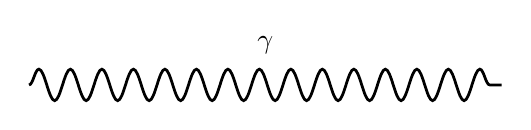
\begin{tikzpicture}
    % Draw a wavy line representing a gamma particle
    \draw[decorate, decoration={snake, amplitude=2mm, segment length=4mm}, line width=1pt] (0,0) -- (6,0);
    % Add a label to indicate that it's a gamma particle
    \node at (3, 0.5) {$\gamma$};
\end{tikzpicture}

\end{document}